\subsection{Current and future automotive architecture}
\label{sec:architectures}
Modern vehicles are mostly electrically or electronically controlled, ranging from basic functionality such as accelerating and controlling the lights, to more advanced features such as ride height control through a touch screen or autonomous emergency braking. New European legislation will mandate even more of those functions such as an alcohol interlock, driver drowsiness detection, event data recorders and more. Each function is implemented with one or more dedicated electronic control units (ECUs). The ECUs need to communicate together to achieve a certain function and often need to interface with other functions for data or to achieve a certain safety requirement. The current electrical/electronic control architecture is decentralized, and the networks are grouped based on function. For example a drivetrain network or a body control network. In practice vehicles can have more than 100 ECUs~\cite{bandur2021making} and several communication networks. This has several drawbacks, among others: increased communication load on the network, increased costs, increased software complexity, more software variants, higher maintenance costs and reduced reliability~\cite{bandur2021making}. An example of a decentralized function based architecture can be found in Figure~\ref{fig:functional-arch}, the blue rectangles represent ECUs, ECUs that are part of a single function or domain (body control, drivetrain etc) are connected to each other with an automotive network such as LIN or CAN. The functions or domains work together by means of a gateway (red rectangle) which bridges or translates messages to and from the different networks. Sometimes certain ECUs are also connected to more than one network for practical reasons such as the Steering column ECU in the example.

\begin{figure}[htb]
    \centering
    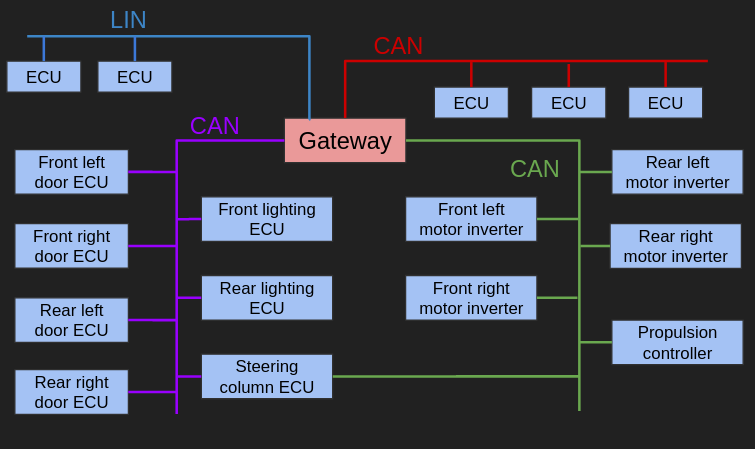
\includegraphics[width=\textwidth]{images/functional-arch.png}
    \caption{Example of an automotive decentralized control architecture}
    \label{fig:functional-arch}
\end{figure}

The rise of advanced driver assistance systems (ADAS) requiring more network bandwidth, extra functions required by European legislation and the aforementioned drawbacks has lead the industry to chose a centralized control architecture with an Ethernet based communication network as the future electrical/electronic architecture, commonly called the zonal architecture~\cite{ashjaei2021time}. Instead of having many small ECUs performing only part of a single function, in the zonal architecture there will be one central ECU responsible for all the control functions and a few larger ECUs, called zone ECUs, which execute the commands of the ECUs. The zone ECUs are strategically placed to handle all functions in the physical neighbourhood of the ECU. To reduce complexity, weight, cost and support ADAS functions, the ECUs are networked through a single high bandwidth, low latency network instead of multiple low bandwidth networks. To ease this transition a zone ECU can act as a bridge for legacy networks used by legacy components in its physical neighbourhood. An example of the zonal architecture with a zone ECU acting as a bridge for a legacy component is shown in Figure~\ref{fig:zonal-arch}

In the new zonal architecture the zone ECU and central controller communicate using a high bandwidth low latency network, automotive Ethernet (single twisted pair physical layer) together with Time Sensitive Networking (TSN) have been chosen as the key networking technologies. The choice for automotive Ethernet is supported by the work of the Time Sensitive Networking (TSN) Task Group of the IEEE 802.1 Working Group, which allow real-time communication over IEEE 802.3 (Ethernet) networks~\cite{klaus2019zonal}. Other relevant factors for choosing automotive Ethernet and TSN are the high bandwidth capabilities relative to traditional networks such as CAN and FlexRay, Internet Protocol (IP) based end-to-end communication support, automotive specific physical layer standards for various data rates, and standardization by the IEEE~\cite{ashjaei2021time}.

\begin{figure}[htb]
    \centering
    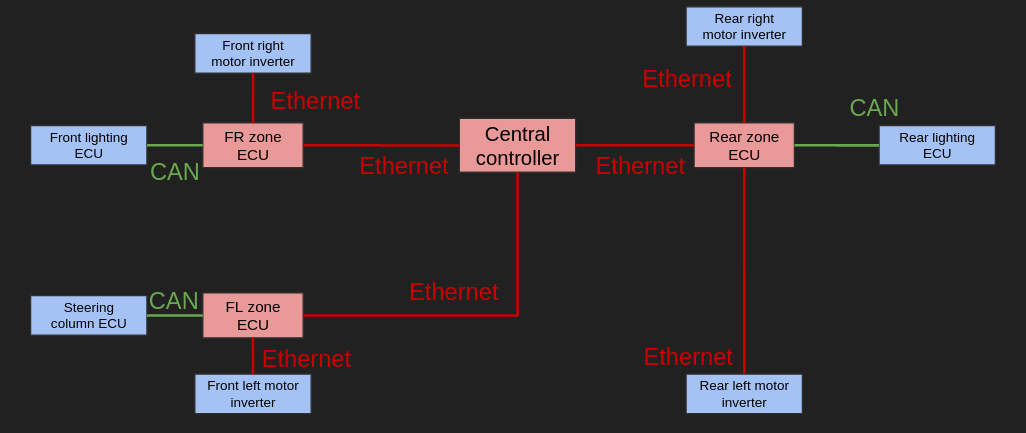
\includegraphics[width=\textwidth]{images/zone-arch.png}
    \caption{Example of an automotive zonal architecture}
    \label{fig:zonal-arch}
\end{figure}

The same vehicle is represented in Figure~\ref{fig:functional-arch} as in Figure~\ref{fig:zonal-arch} but with a decentralized functional architecture and a centralized zonal architecture respectively. The number of ECUs is reduced from 18 to 11 respectively, which is achieved by consolidating ECUs into the zone ECUs, reducing mass. The total number of networks stayed the same, but crucially the physical wiring loom has been simplified in the zonal architecture as there is only a single network going from the back to the front of the vehicle, reducing weight and costs as short wire harnesses can be manufactured automatically.